\documentclass[11pt]{article}
% Author : liambeguin
%
% Usage :
%
% \documentclass[11pt]{article}
% % Author : liambeguin
%
% Usage :
%
% \documentclass[11pt]{article}
% % Author : liambeguin
%
% Usage :
%
% \documentclass[11pt]{article}
% \input{ets_page.tex}
% \EtsPageCourse{ELE778-01}
%	{Intelligence artificielle: r\'eseaux neuroniques et syst\`emes experts}
% \EtsPageTitle{Laboratoire 2}
% \EtsPageProf{Cynthia}{Moussa}
% \EtsPageAuthA{Liam}{Beguin}{BEGL02129304}
% \EtsPageAuthB{Louis}{Laporte}{LAPL14128903}
% \EtsPageAuthC{}{}{}
%
% \begin{document}
% \MakeEtsPage
% \end{document}

\usepackage[french]{babel}
\usepackage[utf8]{inputenc}
\usepackage{tikz}
\usepackage{pgf}
\usetikzlibrary{arrows,automata}
\usepackage[left=2cm, right=2cm]{geometry}
\usepackage{amsmath,amsfonts,amssymb}
\usepackage{listings}

\newcommand{\EtsPageCourse}[2]{\renewcommand{\EtsPageCourse}{
	\textsc{\textbf{\Huge #1 - #2}}
}}
\newcommand{\EtsPageTitle} [1]{\renewcommand{\EtsPageTitle}{
	\textsc{\Large #1 }
}}
\newcommand{\EtsPageProf}  [2]{\renewcommand{\EtsPageProf}{
			\textsc{\Large Pr\'esent\'e \`a : \\
			#1 \textsc{#2}}
}}
\newcommand{\EtsPageAuthA} [3]{\renewcommand{\EtsPageAuthA}{
	\large #1 \textsc{#2} \\\emph{#3}
}}
\newcommand{\EtsPageAuthB} [3]{\renewcommand{\EtsPageAuthB}{
	\large #1 \textsc{#2} \\\emph{#3}
}}
\newcommand{\EtsPageAuthC} [3]{\renewcommand{\EtsPageAuthC}{
	\large #1 \textsc{#2} \\\emph{#3}
}}

\newcommand{\HRule}{\rule{\linewidth}{0.5mm}}

\newcommand{\EtsPageGenerate}{
	\begin{titlepage}
		\begin{center}
			\vspace{5cm}
			\EtsPageCourse
			\vspace{2cm}

			\EtsPageTitle
			\vspace{2.5cm}

			\EtsPageProf
			\vspace{1.5cm}

			% Bottom of the page
			\vfill
			% Authors
			\begin{minipage}{0.4\textwidth}
				\begin{flushleft}
					\EtsPageAuthA
				\end{flushleft}
			\end{minipage}
			\begin{minipage}{0.4\textwidth}
				\begin{flushright}
					\EtsPageAuthB
				\end{flushright}
			\end{minipage}
			\begin{minipage}{0.4\textwidth}
				\begin{center}
					\EtsPageAuthC
				\end{center}
			\end{minipage}

			\vspace{2cm}
			\HRule \\[0.4cm]
			{ \huge \bfseries \'Ecole de technologie superieure \\[0.4cm] }
			\HRule \\[1.5cm]
			\vspace{1.5cm}

			%date
			{\large \today}
		\end{center}
	\end{titlepage}
}

% \EtsPageCourse{ELE778-01}
%	{Intelligence artificielle: r\'eseaux neuroniques et syst\`emes experts}
% \EtsPageTitle{Laboratoire 2}
% \EtsPageProf{Cynthia}{Moussa}
% \EtsPageAuthA{Liam}{Beguin}{BEGL02129304}
% \EtsPageAuthB{Louis}{Laporte}{LAPL14128903}
% \EtsPageAuthC{}{}{}
%
% \begin{document}
% \MakeEtsPage
% \end{document}

\usepackage[french]{babel}
\usepackage[utf8]{inputenc}
\usepackage{tikz}
\usepackage{pgf}
\usetikzlibrary{arrows,automata}
\usepackage[left=2cm, right=2cm]{geometry}
\usepackage{amsmath,amsfonts,amssymb}
\usepackage{listings}

\newcommand{\EtsPageCourse}[2]{\renewcommand{\EtsPageCourse}{
	\textsc{\textbf{\Huge #1 - #2}}
}}
\newcommand{\EtsPageTitle} [1]{\renewcommand{\EtsPageTitle}{
	\textsc{\Large #1 }
}}
\newcommand{\EtsPageProf}  [2]{\renewcommand{\EtsPageProf}{
			\textsc{\Large Pr\'esent\'e \`a : \\
			#1 \textsc{#2}}
}}
\newcommand{\EtsPageAuthA} [3]{\renewcommand{\EtsPageAuthA}{
	\large #1 \textsc{#2} \\\emph{#3}
}}
\newcommand{\EtsPageAuthB} [3]{\renewcommand{\EtsPageAuthB}{
	\large #1 \textsc{#2} \\\emph{#3}
}}
\newcommand{\EtsPageAuthC} [3]{\renewcommand{\EtsPageAuthC}{
	\large #1 \textsc{#2} \\\emph{#3}
}}

\newcommand{\HRule}{\rule{\linewidth}{0.5mm}}

\newcommand{\EtsPageGenerate}{
	\begin{titlepage}
		\begin{center}
			\vspace{5cm}
			\EtsPageCourse
			\vspace{2cm}

			\EtsPageTitle
			\vspace{2.5cm}

			\EtsPageProf
			\vspace{1.5cm}

			% Bottom of the page
			\vfill
			% Authors
			\begin{minipage}{0.4\textwidth}
				\begin{flushleft}
					\EtsPageAuthA
				\end{flushleft}
			\end{minipage}
			\begin{minipage}{0.4\textwidth}
				\begin{flushright}
					\EtsPageAuthB
				\end{flushright}
			\end{minipage}
			\begin{minipage}{0.4\textwidth}
				\begin{center}
					\EtsPageAuthC
				\end{center}
			\end{minipage}

			\vspace{2cm}
			\HRule \\[0.4cm]
			{ \huge \bfseries \'Ecole de technologie superieure \\[0.4cm] }
			\HRule \\[1.5cm]
			\vspace{1.5cm}

			%date
			{\large \today}
		\end{center}
	\end{titlepage}
}

% \EtsPageCourse{ELE778-01}
%	{Intelligence artificielle: r\'eseaux neuroniques et syst\`emes experts}
% \EtsPageTitle{Laboratoire 2}
% \EtsPageProf{Cynthia}{Moussa}
% \EtsPageAuthA{Liam}{Beguin}{BEGL02129304}
% \EtsPageAuthB{Louis}{Laporte}{LAPL14128903}
% \EtsPageAuthC{}{}{}
%
% \begin{document}
% \MakeEtsPage
% \end{document}

\usepackage[french]{babel}
\usepackage[utf8]{inputenc}
\usepackage{tikz}
\usepackage{pgf}
\usetikzlibrary{arrows,automata}
\usepackage[left=2cm, right=2cm]{geometry}
\usepackage{amsmath,amsfonts,amssymb}
\usepackage{listings}

\newcommand{\EtsPageCourse}[2]{\renewcommand{\EtsPageCourse}{
	\textsc{\textbf{\Huge #1 - #2}}
}}
\newcommand{\EtsPageTitle} [1]{\renewcommand{\EtsPageTitle}{
	\textsc{\Large #1 }
}}
\newcommand{\EtsPageProf}  [2]{\renewcommand{\EtsPageProf}{
			\textsc{\Large Pr\'esent\'e \`a : \\
			#1 \textsc{#2}}
}}
\newcommand{\EtsPageAuthA} [3]{\renewcommand{\EtsPageAuthA}{
	\large #1 \textsc{#2} \\\emph{#3}
}}
\newcommand{\EtsPageAuthB} [3]{\renewcommand{\EtsPageAuthB}{
	\large #1 \textsc{#2} \\\emph{#3}
}}
\newcommand{\EtsPageAuthC} [3]{\renewcommand{\EtsPageAuthC}{
	\large #1 \textsc{#2} \\\emph{#3}
}}

\newcommand{\HRule}{\rule{\linewidth}{0.5mm}}

\newcommand{\EtsPageGenerate}{
	\begin{titlepage}
		\begin{center}
			\vspace{5cm}
			\EtsPageCourse
			\vspace{2cm}

			\EtsPageTitle
			\vspace{2.5cm}

			\EtsPageProf
			\vspace{1.5cm}

			% Bottom of the page
			\vfill
			% Authors
			\begin{minipage}{0.4\textwidth}
				\begin{flushleft}
					\EtsPageAuthA
				\end{flushleft}
			\end{minipage}
			\begin{minipage}{0.4\textwidth}
				\begin{flushright}
					\EtsPageAuthB
				\end{flushright}
			\end{minipage}
			\begin{minipage}{0.4\textwidth}
				\begin{center}
					\EtsPageAuthC
				\end{center}
			\end{minipage}

			\vspace{2cm}
			\HRule \\[0.4cm]
			{ \huge \bfseries \'Ecole de technologie superieure \\[0.4cm] }
			\HRule \\[1.5cm]
			\vspace{1.5cm}

			%date
			{\large \today}
		\end{center}
	\end{titlepage}
}


\usepackage{graphicx}
\usepackage{multirow}
\usepackage{color, colortbl}
\usepackage[
	pdftitle   ={ELE778 rapport de laboratoire 2.2},
	pdfsubject ={Detail de l'implementation d'un reseau de Neurones a
		retro-propagation du gradient d'erreur},
	pdfauthor  ={Liam BEGUIN - Louis LAPORTE},
	pdfkeywords={Neural network, mini-batch SGD, TiDigits classification},
]{hyperref} % Required for links
\usepackage{enumitem}



\EtsPageCourse{ELE778-01}
	{Intelligence artificielle: r\'eseaux neuroniques et syst\`emes experts}
\EtsPageTitle{Laboratoire 2}
\EtsPageProf{Cynthia}{Moussa}
\EtsPageAuthA{Liam}{Beguin}{BEGL02129304}
\EtsPageAuthB{Louis}{Laporte}{LAPL14128903}
\EtsPageAuthC{}{}{}

\begin{document}
\EtsPageGenerate
\tableofcontents

\newpage
\section{Notations et symboles}
\begin{tabular}{p{1.75cm}p{10cm}}
	${\bf x}$ & Entr\'ee du r\'eseau, \\
	${\bf y_x}$ & Sortie attendue du r\'eseau pour l'entr\'ee {\bf x}, \\
	${\bf \hat y_x}$ & Pr\'ediction du r\'eseau pour l'entr\'ee {\bf x}, \\
	${\bf a} \circ {\bf b}$ & Produit matriciel de
		\href{https://en.wikipedia.org/wiki/Hadamard_product_(matrices)}
		{Hadamard}, \\
	$\epsilon_{\bf x}$ & taux d'erreur lorsque le r\'eseau evalue l'entree ${\bf x}$, \\
	$\sigma(z)$ & Fonction d'activation generique, \\
	$\sigma'(z)$ & Deriv\'ee de la fonction d'activation, \\
	$C(w, b)$ & Fonction de cout g\'en\'erique, \\
	${\bf C}'(w, b)$ & D\'eriv\'ee de la fonction de cout g\'en\'erique par
		rapport a ${\bf \hat y}$, \\
	$\nabla_bC$ & \href{https://en.wikipedia.org/wiki/Matrix_calculus}
		{D\'eriv\'ees de $C$} par rapport aux seuils de la couche $(l)$, \\
	$\nabla_wC$ & D\'eriv\'ees de $C$ par rapport aux poids de la couche $(l)$, \\
	$d^{(l)}$ & Nombre d'elements sur la couche $(l)$, \\
	${\bf w}^{(l)}(T)$ & Ensemble des poids de la couche $(l)$ \`a l'\'epoque $T$, \\
\end{tabular}
\newpage



\section{Introduction}
Après avoir fait une étape de pré-traitement lors du laboratoire 2.1, nous
allons maintenant implémenter un r\'eseau de neurones \`a r\'etro-propagation du
gradient d’erreur dans le but de classifier, le plus précisément possible,
le dataset {\em TiDigits} (english spoken digits from 1 to 9).

Pour implémenter ce r\'eseau de neurones, nous utiliserons {\em Python}.
Voici une liste d'avantages versus inconv\'enients qui ont motiv\'e notre choix
pour ce language :
\begin{itemize}
	\item Avantages:
		\subitem Rapidit\'e de d\'eveloppement,
		\subitem Language interpr\'et\'e donc pas de compilation,
		\subitem Modules de calcul matriciel performants,
		\subitem Language accessible.
	\item Inconvenients:
		\subitem Language interpr\'et\'e donc moins rapide. \\
\end{itemize}

Dans un premier temps, nous entrainerons le r\'eseau sur un set de donn\'ees puis
nous \'evaluerons sa capacit\'e a g\'en\'eraliser sur de nouvelles donn\'ees non utilis\'ees
lors de l'entrainement.

\section{Impl\'ementation du r\'eseau de neurones}
\subsection{Architecture globale}
\begin{figure}[htp]
	\centering
	\includegraphics[scale=.5]{img/neuron.png}
	\caption{Repr\'esentation symbolique d'un neurone.}
\end{figure}

Comme dit en introduction, Nous allons impl\'ementer un r\'eseau de neurones a
r\'etro-propagation du gradient d'erreur. Ici, nous \'enoncerons les notations et
\'equations g\'en\'eriques utilis\'ees au sein du r\'eseau.

La majorit\'e des calculs sont effectu\'es sous forme matricielle afin de simplifier
et g\'en\'eraliser les \'equations mais aussi de mieux tirer avantage des ressources
de calcul disponibles.

\'Etant donn\'e que le r\'eseau doit \^etre tr\`es flexible quant au nombre de
couches et au nombre de neurones, nous utiliserons un tuple (une liste
invariante) pour instancier le r\'eseau.
Chaque \'el\'ement de la liste repr\'esente une couche du r\'eseau
(incluant la couche d'entr\'ee) et sa valeur d\'etermine le nombre de neurones
present sur la couche.
Pour la couche de sortie, nous utiliserons un vecteur de
type \emph{one-hot} ou un seul element est actif \`a la fois.

D'autre part, on nous demande aussi que le r\'eseau soit capable d'utiliser
differentes fonctions d'activation. Base sur cette contrainte, nous avons
choisi d'aussi donner a l'utilisateur la possibilite de choisir entre
differentes fonctions de cout et differentes fonctions de r\'egularisation.

\paragraph{Notations: }Soit, $w_{jk}^{(l)}$ le poid connectant le neurone $k$
de la couche $(l-1)$ au neurone $j$ de la couche $(l)$, o\`u :
$$
\left \{
	\begin{aligned}
		&1 \le l \le L         &\qquad \text{layers} \\
		&0 \le k \le d^{(l-1)} &\qquad \text{inputs} \\
		&1 \le j \le d^{(l)}   &\qquad \text{outputs}\\
	\end{aligned}
\right .
$$
On d\'efinit donc ${\bf w}^{(l)}$ la matrice de dimension $\Big((l) \times (l-1)\Big)$
connectant la couche $(l-1)$ \`a la couche $(l)$ cr\'eant ainsi, $(L-1)$ matrices
de poids sur l'ensemble du r\'eseau. \\
\paragraph{Feedforward:} cette \'etape propage l'entr\'ee a travers l'ensemble du
r\'eseau et enregistre toutes les variables intermediaires.
\begin{equation}
	\begin{aligned}
		z_j^{(l)} &= \sum_k^{d^{(l-1)}{w_{jk}^{(l)}}} \cdot a_{k}^{(l-1)} + b_{j}^{(l)}\\
		{\bf z}_x^{(l)} &= {\bf w}^{(l)} \cdot {\bf a}_x^{(l-1)} + {\bf b}^{(l)}\\
		{\bf a}_x^{(l)} &= \sigma\left({\bf z}_x^{(l)}\right)\\
	\end{aligned}
\end{equation}
Pour avoir la pr\'ediction finale du r\'eseau ${\bf \hat{y}}$, il faut r\'ep\'eter l'\'etape
ci-dessus jusqu'\`a atteindre la sortie o\`u on obtient:
\begin{equation}
	\begin{aligned}
		{\bf z}_x^{(L)} &= {\bf w}^{(L)} \cdot {\bf a}_x^{(L-1)} + {\bf b}^{(L)}\\
		{\bf \hat{y}}_x &= \sigma\left({\bf z}_x^{(L)}\right)\\
	\end{aligned}
\end{equation}

\paragraph{La fonction de cout}est la fonction utilis\'ee lors du processus
d'entrainement pour \'evaluer l'erreur entre la pr\'ediction du r\'eseau
${\bf \hat{y}}$ et la sortie attendue ${\bf y}$. Les diff\'erents fonctions
disponibles seront detaill\'ees dans la section \ref{cost}.
Pour la suite, nous l'appelerons de fa\c con generique: $C({\bf w}, {\bf b})$.

\paragraph{La fonction de regularization}est la fonction utilisee lors du processus
d'entrainement pour p\'enaliser la minimisation de la fonction de cout. Ceci sera
couvert plus en detail dans la section \ref{overfitting}.
Pour la suite, nous l'appelerons de fa\c con g\'en\'erique: $\Omega({\bf w})$.

\paragraph{retro-propagation:} Cette \'etape calcule l'impacte de chaque poids
(et seuil) sur l'erreur finale. Pour obtenir l'erreur $\delta_j^l$ due au neurone
$j$ de la couche $l$, il faut propager l'erreur de la sortie vers l'entr\'ee
avec les \'equations suivantes:

\begin{equation}
	\begin{aligned}
		{\boldsymbol \delta}^{(L)} &= \frac{\partial C}{\partial {\bf z}^{(L)}} =
		\frac{\partial C}{\partial {\bf a}^{(L)}} \circ \frac{\partial {\bf a}^{(L)}}{\partial {\bf z}^{(L)}} \\
		&= \frac{\partial C}{\partial {\bf a}^{(L)}} \circ \sigma'\left({\bf z}^{(L)}\right)
		= \frac{\partial C}{\partial {\bf \hat y}} \circ \sigma'\left({\bf z}^{(L)}\right)\\
		&= C'({\bf w}, {\bf b}) \circ \sigma'\left({\bf z}^{(L)}\right)\\
	\end{aligned}
\end{equation}

De la m\^eme mani\`ere, on d\'efinit une notation r\'ecursive:
\begin{equation}
	\begin{aligned}
		\delta_j^{(l)} &= \frac{\partial C}{\partial z_j^{(l)}} =
		\sum_k{\frac{\partial C}{\partial z_k^{(l+1)}} \cdot
		\frac{\partial z_k^{(l+1)}}{\partial z_j^{(l)}}} \\
		&= \sum_k\delta_k^{(l+1)} \cdot \frac{\partial z_k^{(l+1)}}{\partial z_j^{(l)}} \\
	\end{aligned}
\end{equation}
Or,
$$
	z_k^{(l+1)} = \sum_j^{d^{(l)}}{w_{jk}^{(l+1)}\cdot a_j^{(l)} + b_k^{(l+1)}}\\
$$
Donc,
$$
	\frac{\partial z_k^{(l+1)}}{\partial z_j^l} =
	w_{kj}^{(l+1)}\cdot \sigma'\left( z_j^{(l)}\right)\\
$$
Et,
$$
	\delta_j^{(l)} = \sigma'\left( z_j^{(l)}\right)\cdot \sum_k\delta_k^{(l+1)} \cdot
	w_{kj}^{(l+1)} \\
$$
Nous pouvons maintenant utiliser $\delta_{j}^{(l)}$ pour determiner
l'impacte de chaque seuil sur la fonction de cout:
\begin{equation}
	\begin{aligned}
		\frac{\partial C}{\partial b_j^{(l)}} &= \frac{\partial C}{\partial z_j^{(l)}}
		\cdot \frac{\partial z_j^{(l)}}{\partial b_j^{(l)}} \\
		&= \delta_j^{(l)}  \\
	\end{aligned}
\end{equation}
Idem pour les poids:
\begin{equation}
	\begin{aligned}
		\frac{\partial C}{\partial w_{jk}^{(l)}} &= \frac{\partial C}{\partial z_j^{(l)}}
		\cdot\frac{\partial z_j^{(l)}}{\partial w_{jk}^{(l)}} = \delta_j^{(l)}
		\cdot \frac{\partial z_j^{(l)}}{\partial w_{jk}^{(l)}} =
		\delta_j^{(l)} \cdot a_{k}^{(l-1)} \\
		&= \delta_j^{(l)} \cdot	\sigma\left(z_{k}^{(l-1)} \right)
	\end{aligned}
\end{equation}
Et sous formes matricielles:
\begin{equation}
	\begin{aligned}
		\boldsymbol \delta^{(l)} &= \left(\left({\bf w}^{(l+1)} \right)^{T}
		\cdot \boldsymbol \delta^{(l+1)} \right)
		\circ \sigma'\left( {\bf z}^{(l)}\right) \\
		\nabla_bC = \frac{\partial C}{\partial {\bf b}^{(l)}} &=
		\boldsymbol\delta^{(l)}  \\
		\nabla_wC = \frac{\partial C}{\partial {\bf w}^{(l)}} &=
		\boldsymbol\delta^{(l)} \cdot \left(\sigma\left({\bf z}^{(l-1)}\right)\right)^{T}\\
	\end{aligned}
\end{equation}

\paragraph{Actualisation des poids:} maintenant que le r\'eseau est en mesure de
quantifier l'erreur due a chaque neurone, nous pouvons mettre a jour les poids
\`a l'aide des expressions suivantes:
\begin{equation}
	\begin{aligned}
		{\bf b}^{(l)}(T+1) &= {\bf b}^{(l)}(T) - \eta \nabla_bC \\
		{\bf w}^{(l)}(T+1) &= {\bf w}^{(l)}(T) - \eta \cdot \bigg( \nabla_bC + \Omega'({\bf w})\bigg)\\
	\end{aligned}
\end{equation}



\subsection{Extraction des donn\'ees}
% TODO
% preprocessing, chx du 40, 50 ,60
% normalisation du dataset
% classification homme / femme

\begin{figure}[h]
	\centering
	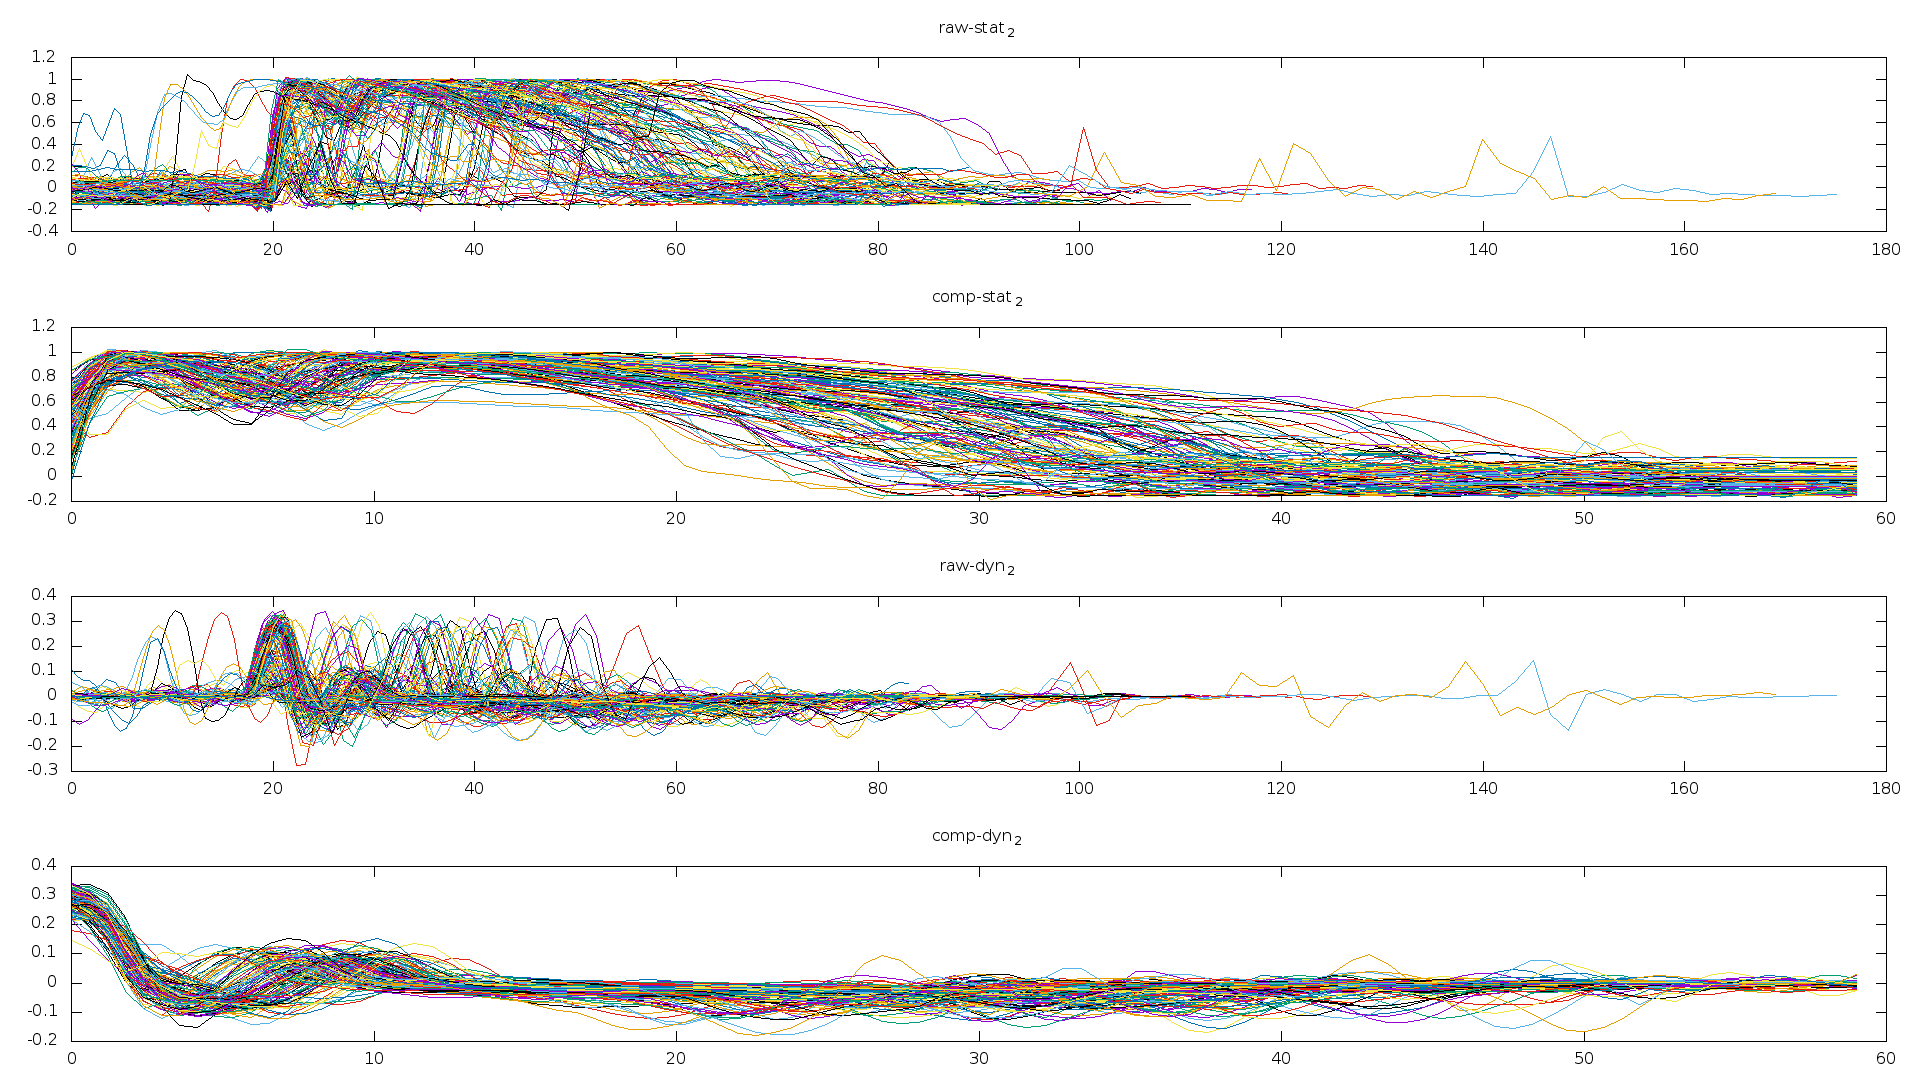
\includegraphics[scale=.3]{img/preprocessing.png}
	\caption{Repr\'esentation des \'en\'ergies statiques et dynamiques avant et
	apr\`es le traitement}
\end{figure}

Pour extraire les informations de la base de donn\'ee {\em TiDigits}, nous avons
utilis\'e le code que nous avions d\'evelopp\'e pour la premi\`ere partie du laboratoire.
Nous nous sommes bas\'es sur les similarit\'es entre la prononciation d'un
m\^eme chiffre par plusieurs individus. Pour cela, nous avons filtr\'e
les \'energies statiques et dynamiques afin de pouvoir accentuer les
propri\'et\'es de chaque chiffre.


Le filtrage consiste dans un premier temps \`a utiliser une op\'eration de
seuillage sur l'\'energie statique afin de d'\'et\'ecter le d\'ebut du mot et
d'\'eliminer tout le {\em blanc} qui se trouve au d\'ebut de l'enregistrement.
La seconde \'etape permet d'aligner le d\'ebut de chaque mot en utilisant le
premier maximum de l'\'energie dynamique.
Ceci nous permet de ne pas \^etre trop sensible aux diff\'erences d'attaque
entre les individus.

Comme tous les fichiers n'ont pas la m\^eme taille, nous devons ajouter
du padding afin que les donn\'ees puissent \^etre utilis\'ees comme
entr\'ee pour le r\'eseau. En effet, dans le cas o\`u les longueurs ne sont pas
identiques, il est impossible d'alimenter le r\'eseau en raison d'erreurs
de dimensions sur les produits matriciels.
D'autre part, dans le but d'am\'eliorer la vitesse de convergence de
l'apprentissage et de limiter la complexit\'e du mod\`ele, nous avons choisi de
ne garder que les donn\'ees statiques et de les normaliser, selon chaque colonne.
La figure \ref{fig:w_prep} donne un aper\c cu de l'impacte du pr\'e-traitement
sur les performances du r\'eseau.

La fonction d'extraction des donn\'ees {\em extract\_datasets()}
est con\c{c}ue pour prendre 2 param\`etres: le nombre de features d\'esir\'e
(40, 50, 60, ...) et un bool\'een permettant de choisir si l'on desir ou non
classifier selon le sexe de l'interpr\`ete. cette fonction retourne 3 listes:
un {\em training\_set}, un {\em validation\_set} et un {\em test\_set} o\`u
chaque \'el\'ement est une combinaison de 2 vecteurs les features {\bf x} et les
labels {\bf y}.

\lstset{tabsize = 4,
frame=lines,
numbers=left,
captionpos=b,
caption = {Fonction appele\'e pour extraire les donn\'ees d'un unique fichier},
language = python,
basicstyle=\small}
\begin{lstlisting}
def extract_sample(file_, size=60, sex=False, out_size=9):
    # Preprocess file ...
    x = prep.Preprocessing(file_, size)
    x.start_point_detection(threshold=0.5, n=10)
    x.cut_first_max(n=20)
    x.normalize()
    x.fit()
    x.get_subset('static')

    num = int(re.search(r'(?=.*)[0-9](?=.*)', file_).group(0))

    # make a column of the whole array
    features = x.data.reshape((len(x.data)*len(x.data[0]), 1) )

    if sex:
        if re.search(r'.*woman.*', file_):
            labels = vectorize_output( num - 1 + out_size, shape=(out_size*2, 1))
        else:
            labels = vectorize_output(num-1, shape=(out_size*2, 1))
    else:
        labels = vectorize_output(num-1, shape=(out_size, 1))

    return (features, labels)

\end{lstlisting}

\subsection{Initialisation du r\'eseau}
Lorsque le r\'eseau est instanci\'e, les param\`etres tels que $\eta$ et $\lambda$
sont copi\'es dans l'object \emph{Network} et les matrices de poids et de
seuils (\emph{weights} et \emph{biases}) sont g\'en\'er\'ees. Les dimensions
de ces matrices sont determin\'ees en fonction du nombre de neurones sur chaque
couche et du nombre de couches $L$.


D'autre part, du fait que la fonction al\'eatoire utilis\'ee pour l'initialisation
des poids donne une distribution avec les param\`etres suivants $\mu=0$ et $\sigma=1$,
l'initialisation des poids a tendance \`a saturer les neurones et ralentire l'apprentissage.
car :
\begin{equation}
	\begin{aligned}
		Var(z) &= \sum_{i=1}^N(Var(x_i)) \\
		Var(z) &= N \cdot Var(x) \\
		\sigma(z) &= \sqrt{N} \cdot 1 \\
		\sigma(z) &= \sqrt{N}
	\end{aligned}
\end{equation}

\begin{figure}[htp]
	\centering
	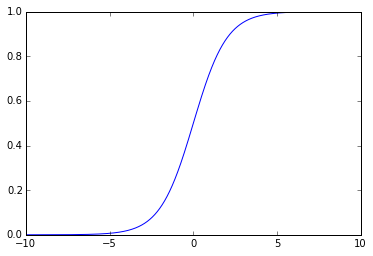
\includegraphics[scale=.5]{img/sigmoid_sat.png}
	\caption{Visualisation de la saturation de la fonction \emph{sigmoid} si
	$|z| \ge 5$.}
\end{figure}

Pour contrer cette saturation et donc accelerer les premi\`eres \'epoques
d'apprentissage, nous utiliserons une distribution plus \'etroite avec les
param\`etres $\mu=0$ et $\sigma =1/\sqrt{N}$ \\


\lstset{tabsize = 4,
frame=lines,
numbers=left,
captionpos=b,
caption = {Initialisation des poids et seuils},
language = python,
basicstyle=\small}
\begin{lstlisting}
self.biases  = [ np.random.randn(y, 1) for y in struct[1:] ]
self.weights = [ np.random.randn(y, x) / np.sqrt(x) \
				for x, y in zip(struct[:-1], struct[1:]) ]
\end{lstlisting}

\newpage
\subsection{Fonctions d'activation}
% http://tflearn.org/activations/
\paragraph{La fonction sigmoid} est la fonctions de r\'ef\'erence dans les r\'eseaux de
neurones et est definie de la mani\`ere suivante: \\
\begin{equation}
	\begin{aligned}
		\sigma(x)  &= \frac{1}{1+e^{-x}} \\
		\sigma'(x) &= \sigma(x)(1-\sigma(x))
	\end{aligned}
\end{equation}
\begin{figure}[htp]
	\centering
	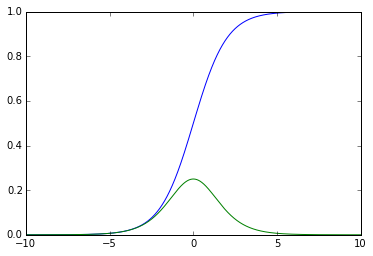
\includegraphics[scale=.5]{img/act_sigmoid.png}
	\caption{Representation de la fonction sigmoid (blue) et de sa derivee (vert)}
\end{figure}

elle permet de d'obtenir une sortie comprise dans l'intervalle [0;1] qui peut
dans certain cas \^etre assimil\'e \`a une probabilit\'e. C'est principalement
cette fonction que nous utiliserons.

\lstset{tabsize = 4,
frame=lines,
numbers=left,
captionpos=b,
caption = {Definition de la fonction {\em sigmoid} et de sa d\'eriv\'ee},
language = python,
basicstyle=\small}
\begin{lstlisting}
def sigmoid(z, prime=False):
    if prime:
		return sigmoid(z)*(1-sigmoid(z))
	else:
		return 1.0 / (1.0 + np.exp(np.negative(np.clip(z, -50, 50))))
\end{lstlisting}

\newpage
\paragraph{La fonction tangente hyperbolique} est aussi tres rependue dans les
r\'eseau de neurones et permet de definir un {\em soft threshold}. En d'autres termes,
c'est une version derivable de la fonction de seuil utilisee par le perceptron.
Elle se comporte comme une fonction lin\'eaire proche de 0 et comme une fonction
de seuil sur le reste de son ensemble de d\'efinition.
Elle est d\'efinie de la mani\`ere suivante:
\begin{equation}
	\begin{aligned}
		\tanh(x)  &= \frac{\sinh(x)}{\cosh(x)} \\
		\tanh'(x) &= 1-\tanh^2(x)
	\end{aligned}
\end{equation}
\begin{figure}[htp]
	\centering
	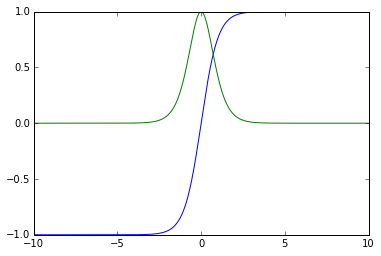
\includegraphics[scale=.5]{img/act_tanh.png}
	\caption{Repr\`esentation de la fonction tanh (blue) et de sa deriv\'ee (vert)}
\end{figure}
\begin{equation}
\end{equation}

\lstset{tabsize = 4,
frame=lines,
numbers=left,
captionpos=b,
caption = {D\'efinition de la fonction tanh et de sa deriv\'ee},
language = python,
basicstyle=\small}
\begin{lstlisting}
def tanh(z, prime=False):
    if prime:
		return 1.0 - np.square(tanh(z))
	else:
		return np.tanh(z)
\end{lstlisting}

\newpage
\paragraph{La fonction Softplus} est quant \`a elle beaucoup moins utilis\'ee mais
semblait int\'eressante au vue de sa simplicit\'e. Elle est d\'efinie de la mani\`ere
suivante :
\begin{equation}
	\begin{aligned}
		f(x)  &= ln(1+e^x) \\
		f'(x) &= \frac{1}{1+e^{-x}}
	\end{aligned}
\end{equation}
\begin{figure}[htp]
	\centering
	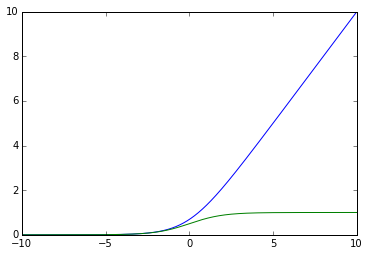
\includegraphics[scale=.5]{img/act_softplus.png}
	\caption{Representation de la fonction softplus (blue) et de sa derivee (vert)}
\end{figure}
\lstset{tabsize = 4,
frame=lines,
numbers=left,
captionpos=b,
caption = {Definition de la fonction {\em softplus} et de sa derivee},
language = python,
basicstyle=\small}
\begin{lstlisting}
def softplus(z, prime=False):
	if prime:
		return sigmoid(z)
	else:
		return np.log(1 + np.exp(np.clip(z, -50, 50)))
\end{lstlisting}


\newpage
\subsection{Fonctions de co\^ut}\label{cost}
Comme \'ennonc\'e pr\'ec\'edemment, nous offrons aussi \`a l'utilisateur la
possibilit\'e de choisir parmis diff\'erentes fonctions de co\^uts, soit la fonction
que le r\'eseau cherche \`a minimiser en ajustant les poids et seuils des connections.
\paragraph{quadratic} est une
\href{https://fr.wikipedia.org/wiki/Erreur_quadratique_moyenne}
{fonction d'erreur quadratique moyenne}. Cete fonction est la plus simple et
est definie de la maniere suivante:
\begin{equation}
	\begin{aligned}
		C(w, b) &= \frac{1}{2\cdot d^{(L)}}\sum_{j}^{d^{(L)}}{({\bf\hat y} - {\bf y})^2}  \\
		{\bf C'}(w, b) &= \frac{1}{d^{(L)}}\cdot({\bf\hat y} - {\bf y})
	\end{aligned}
\end{equation}
\paragraph{cross-entropy} est la seconde option et est implement\'ee dans le but
de limiter le ph\'enom\`ene de \emph{learning slowdown} en \'evitant la saturation des
neurones. Cette fonction permet au r\'eseau de corriger ses poids plus efficacement
dans le cas d'une erreur importante. Elle ne peut \^etre seulement utilis\'ee
avec une fonction d'activation {\em sigmoid} et est construite pour annuler la
multiplication par $\sigma'(z)$ dans l'expression de $\boldsymbol\delta^{(L)}$.
\begin{equation}
	\begin{aligned}
		C(w, b) &= -\frac{1}{d^{(L)}}\sum_{j}^{d^{(L)}}{\left({\bf y}\ln({\bf\hat y}) +
		(1-{\bf y})\ln(1- {\bf \hat y})\right)}  \\
		{\bf C'}(w, b) &= \frac{1}{d^{(L)}}\cdot({\bf\hat y} - {\bf y})
	\end{aligned}
\end{equation}
NOTE: On remarque ici que les d\'eriv\'ees des deux fonctions sont identiques. En
revanche, une condition dans le code est ajout\'ee pour supprimer la multiplication
par $\sigma'(z)$.

\newpage
\subsection{Eviter le sur-ajustement}\label{overfitting}
\begin{figure}[htp]
	\centering
	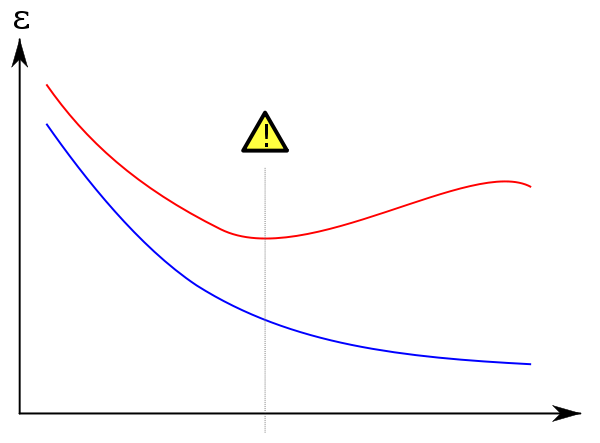
\includegraphics[scale=.4]{img/overfitting.png}
	\caption{erreurs sur le set d'entrainement(bleu) et de validation(rouge)}
\end{figure}
Le sur-ajustement (ou {\em overfitting}) survient lorsque le r\'eseau n'est plus
en train d'apprendre du dataset mais est en train de le m\'emoriser. Ceci se
traduit par un apprentissage trop sp\'ecifique aux donn\'ees, le r\'eseau est
donc en train de mod\'eliser le {\em bruit}. Ceci survient lorsque le mod\`ele
(nombre de neurones et couches) est plus complexe que la fonction \`a
mod\'eliser. Ce sur-apprentissage \`a des cons\'equences n\'efastes sur les
performances du r\'eseau au moment de la g\'en\'eralisation, lorsqu'il est
confront\'e \`a de nouvelles donn\'ees. Il est donc imp\'eratif de le
d\'etecter et de le minimiser.

\paragraph{Validation crois\'ee:} Pour d\'etecter le sur-ajustement, il est
important de s\'eparer le set de donn\'ees en deux une partie pour l'entrainement
l'autre pour la validation. Plusieurs m\'ethodes diff\'erentes sont disponibles
pour d\'eterminer comment s\'eparer le dataset. Plus on \`a de donn\'ees dans le set
d'entrainement plus la pr\'ediction sera bonne mais moins on sera capable de
quantifier la capacit\'e de g\'en\'eralisation du r\'eseau et inversement.

Une m\'ethode int\'eressante \`a citer est le \href{http://work.caltech.edu/slides/slides13.pdf}
{\emph{V-folds} ou \emph{K-folds}} qui permet de maximiser le nombre d'\'echantillons
d'entrainement en divisant le set complet en $V$ sous ensembles. Le r\'eseau est
ensuite entrain\'e sur tous les sous-ensembles moins un qui est utilis\'e pour la
validation (le sous-ensemble de validation est choisi al\'eatoirement et change
\`a chaque \'epoque d'apprentissage). Il faut noter qu'il est important de
s\'electionner les \'echantillons de mani\`ere al\'eatoire afin de ne pas biaiser
l'apprentissage du r\'eseau.

Cependant, notre set de donn\'ees \'etant d\'ej\`a s\'epar\'e en plusieurs sous-ensembles,
nous garderons ces m\'ethodes comme pistes d'am\'elioration futures.

\paragraph{Detection: }Le sur-ajustement peut etre aisement d\'etect\'e lorsque
l'erreur sur le set de validation commence \`a augmenter tandis que l'erreur sur
le set d'entrainement continue de d\'ecroitre.

\paragraph{Early stopping} est une m\'ethode de limitation du sur-ajustement. Elle
consiste \`a monitorer les erreurs au cours de l'entrainement du r\'eseau et
de l'interrompre sous certaines conditions(seuil, moyenne glissante, ...).

\paragraph{Les fonctions de r\'egularisation} sont une autre m\'ethode permettant
de limiter le sur-ajustement. Celles-ci ont pour approche de {\em p\'enaliser}
la minimisation de la fonction d'erreur dans le but d'am\'eliorer la capacit\'e de
g\'en\'eralisation du r\'eseau.

Ici, sont implement\'ees deux des m\'ethodes les plus r\'ependues :
r\'egularisation \emph{L1} et \emph{L2}. Toute deux visent \`a limiter
la magnitude des poids dans l'ensemble du r\'eseau.
Red\'efinissons la fonction de co\^ut de la mani\`ere suivante:
\begin{equation}
	\begin{aligned}
		C({\bf w}, {\bf b}) &= C_0({\bf w}, {\bf b}) + \Omega({\bf w})
	\end{aligned}
\end{equation}

O\`u $\Omega(w)$ est l'expression g\'en\'erale de la fonction de r\'egularization.

On peut maintenant definir $\Omega({\bf w})$ pour chaque type de r\'egularization:
\begin{equation}
	\begin{aligned}
		\Omega_{L1} ({\bf w}) &= \frac{\lambda}{2\cdot d^{(l)}} \cdot \sum{|{\bf w}^{(l)}|}\\
		\boldsymbol\Omega_{L1}'({\bf w}) &= \frac{\lambda}{d^{(l)}} \cdot sign\left ({\bf w}^{(l)} \right)\\
	\end{aligned}
\end{equation}
\begin{equation}
	\begin{aligned}
		\Omega_{L2} ({\bf w}) &= \frac{\lambda}{2\cdot d^{(l)}} \cdot \sum{\left({\bf w}^{(l)}\right) ^2}\\
		\boldsymbol\Omega_{L2}'({\bf w}) &= \frac{\lambda}{d^{(l)}} \cdot {\bf w}^{(l)}\\
	\end{aligned}
\end{equation}
NOTE: \href{http://work.caltech.edu/slides/slides12.pdf}{La r\'egularisation
\emph{Tikhonov}} est une forme generalis\'ee de ces approches et permet une
plus grande flexibilit\'e.

\newpage
\subsection{Entrainement}
L'entrainement du r\'eseau est un processus gourmand en calculs et demandant
beaucoup de ressources. Il est donc important de bien l'optimiser. Dans ce but,
nous sommes pass\'es par plusieurs m\'ethodes avant d'arriver \`a la plus optimale.

\paragraph{batch gradient descent} consiste \`a calculer le gradient en une seule
it\'eration sur l'ensemble des \'echantillons d'entrainement avant de pouvoir
actualiser les poids. Etant donn\'e que l'entrainement n\'ecessite un grand
nombre d'echantillons pour donner des resultats satisfaisant, cette approche
impose des calculs sur des matrices de {\bf grande} dimensions.

\paragraph{stochastic gradient descent : } contrairement \`a la m\'ethode
pr\'ec\'edente, le gradient est ici calcul\'e sur un seul \'echantillon selectionn\'e
al\'eatoirement (d'o\`u son nom). Ceci permet de r\'eduire consid\'erablement le
co\^ut des calculs et est prouv\'e de converger vers la m\^eme valeur que le
{\em batch gradient descent} en montrant que l'esp\'erance math\'ematique des deux
versions du gradient sont \'egales.

\paragraph{Mini-batch stochastic gradient descent} est la m\'ethode impl\'ement\'ee
dans le r\'eseau. Cette version est une g\'en\'eralisation des deux approches
pr\'ec\'edentes. Au lieu de selectionner un seul \'el\'ement al\'eatoirement,
le set d'entrainement est divis\'e en sous ensembles de taille $N$. Il est
int\'er\'essant de noter que si $N=1$, on obtient un {\em stochastic gradient descent}
standard et si $N$ est \'egal \`a la taille du set d'entrainement, on obtient un
{\em batch gradient descent}.

\lstset{tabsize = 4,
frame=lines,
numbers=left,
captionpos=b,
caption = {division du set ${\bf x}$ en sous-ensembles de taille $N$},
language = python,
basicstyle=\small}
\begin{lstlisting}
In [1]: x = [1, 2, 3, 4, 5, 6, 7, 8, 9]
In [2]: N = 2
In [3]: print zip(*[iter(x)]*N)
[(1, 2), (3, 4), (5, 6), (7, 8)]
\end{lstlisting}

Par manque de temps, la r\'etro-propagation impl\'ement\'ee permet seulement de
calculer le gradient sur un \'echantillon unique (un vecteur) et non une matrice
des $N$ \'echantillons. Il faut donc sommer les gradients sur tous les \'el\'ements de
la mini-batch:
$
		\nabla_wC = \sum_{i}^{N}{{\nabla_wC}_i}
$ (Idem pour $\nabla_bC$).

Une impl\'em\'entation 'enti\`erement' matricielle permettrait d'am\'eliorer encore
les performances en exploitant pleinement les capacit\'es de \emph{numpy}
(le module de calcul utilis\'e). Il est aussi int\'eressant de noter que,
si plusieurs CPU sont disponibles, les calculs seront alors {\bf distribu\'es}.
\lstset{tabsize = 4,
frame=lines,
numbers=left,
captionpos=b,
caption = {sommation $N$ des gradients},
language = python,
basicstyle=\small}
\begin{lstlisting}
for x, y in mini_batch:
	# Sum all the gradients over the mini-batch
	self.feedforward(x)
	nabla_bC_i, nabla_wC_i = self.backpropagation(y)
	nabla_bC = np.add(nabla_bC, nabla_bC_i)
	nabla_wC = np.add(nabla_wC, nabla_wC_i)
\end{lstlisting}

\newpage
\subsection{Ajustement des hyper-param\`etres}
% http://neuralnetworksanddeeplearning.com/chap3.html#how_to_choose_a_neural_network's_hyper-parameters
\begin{table}[h]
	\centering

	\begin{tabular}{|c|c|c|c|c|c|c|c|c|c|c|c|c|c|}
		\hline
		dataset & out & $\sigma$  & cost & $\Omega$ & $\eta$ & $\lambda$ &
			epoch  & batch & hidden & tr(\%) & va(\%) & test(\%) & t(s)\\
		\hline
		50 & 18 & s & C & L2 & 0.01 & 0.001 & 5 & 10 & 150 & 59 & 53 & 60 & 11 \\
		\hline
		50 & 18 & s & C & L2 & 0.05 & 0.001 & 5 & 10 & 150 & 38 & 34 & 43  & 10\\
		\hline
		50	& 18 & s & C & L2 & 0.1 & 0.001 & 5 & 10 & 150 & 20 & 15 & 24  & 10\\
		\hline
		50	& 18 & s & C & L2 & 0.5 & 0.001 & 5 & 10 & 150 & 9 & 6 & 16  & 10 \\
		\hline
		50	& 18 & s & C & L2 & 0.5 & 0.001 & 20 & 10 & 20 & 3 & 8 & 15 & 10 \\
		\hline
		50	& 18 & s & C & L2 & 0.5 & 0.001 & 30 & 10 & 0 & 0 & 3 & 12 & 20 \\
		\hline
		\rowcolor{green}
		40	& 18 & s & C & L2 & 0.5 & 0.001 & 30 & 10 & 0 & 0 & 2 & 14 & 20 \\
		\hline
		60	& 18 & s & C & L2 & 0.5 & 0.001 & 30 & 10 & 0 & 0 & 6 & 12 & 20 \\
		\hline
		\rowcolor{green}
		40	& 9 & s & C & L2 & 0.5 & 0.001 & 30 & 10 & 0 & 1 & 1 & 7 & 20 \\
		\hline
		50	& 9 & s & C & L2 & 0.5 & 0.001 & 30 & 10 & 0 & 2 & 1 & 7 & 20 \\
		\hline
		60	& 9 & s & C & L2 & 0.5 & 0.001 & 30 & 10 & 0 & 5 & 1 & 9 & 20 \\
		\hline
		40	& 18 & t & Q & L2 & 0.01 & 0.001 & 30 & 10 & 150 & 12 & 10 & 21 & 40 \\
		\hline
		50	& 18 & t & Q & L2 & 0.01 & 0.001 & 30 & 10 & 150 & 11 & 8 & 20  & 50\\
		\hline
		60	& 18 & t & Q & L2 & 0.01 & 0.001 & 30 & 10 & 150 & 10 & 13 & 21  & 53\\
		\hline
		40	& 9 & t & Q & L2 & 0.01 & 0.001 & 30 & 10 & 50 & 5 & 1 & 10  & 15\\
		\hline
		50	& 9 & t & Q & L2 & 0.01 & 0.001 & 30 & 10 & 50 & 5 & 1 & 12  & 15\\
		\hline
		60	& 9 & t & Q & L2 & 0.01 & 0.001 & 30 & 10 & 50 & 4 & 1 & 11  & 15\\
		\hline
		40	& 18 & sp & Q & L2 & 0.1 & 0.001 & 30 & 10 & 50 & 10 & 6 & 16  & 20\\
		\hline
		50	& 18 & sp & Q & L2 & 0.1 & 0.0001 & 30 & 10 & 50 & 7 & 6 & 15  & 20\\
		\hline
		60	& 18 & sp & Q & L2 & 0.1 & 0.0001 & 30 & 10 & 50 & 7 & 6 & 13  & 20\\
		\hline
		40	& 9 & sp & Q & L2 & 0.01 & 0.0001 & 30 & 10 & 50 & 5 & 1 & 9  & 20\\
		\hline
		50	& 9 & sp & Q & L2 & 0.01 & 0.001 & 30 & 10 & 50 & 5 & 1 & 9  & 20\\
		\hline
		60	& 9 & sp & Q & L2 & 0.01 & 0.001 & 30 & 10 & 50 & 6 & 2 & 9  & 20\\

		\hline
\end{tabular}
  \caption{Tableau r\'ecapitalif des tests effectu\'es sur les
	hyper-param\`etres sur un {\em i5 dual-core, 2.2GHz} }
\end{table}
Pour obtenir la meilleur solution nous avons chercher en premier le
{\em learning rate}  qui donnait la plus petite erreur sur le training set,
ensuite nous avons
ajust\'e le {\em regularization rate} avec un faible nombre d'epochs et pour
finir nous avons ajust\'e le nombre de neurone sur une seule couche cach\'ee.
Les valeurs de sortie 18 et 9 repr\'esentent respectivement avec et sans
classification Homme/Femme.
C repr\'esente la m\'ethode de {\em cross-entropy}, Q la m\'ethode {\em quadratic}
et s, t, sp sont respectivement les fonctions sigmoid, $\tanh$ et softplus.

\newpage
\subsection{Inspection du res\'eau}
Parmis les contraintes obligatoires, il nous est aussi demand\'e de pouvoir
inspecter les couches cach\'ees du r\'eseau. Pour ce faire, nous tirons parti du
fait que {\em Python} est un language interpr\'et\'e et qu'il fournit \`a
l'utilisateur une interface int\'eractive(voir annexe \ref{inspect}).

En combinaison avec la possibilit\'e de savegarder l'\'etat des
objects {\em Network} sous la forme de fichiers (compress\'es ou non), nous
pouvons ais\'ement analyser chaque couche (voir annexe \ref{saveload}).

D'autre part, la conception du r\'eseau permetterai, avec peu d'effort, de coupler
plusieurs objects {\em Network} en un {\em super} r\'eseau.
Ceci pourrai \^etre fait en impl\'ementant les m\'ethodes {\em \_\_add\_\_()}
et {\em \_\_getslice\_\_()} pour respectivement concat\'ener et couper des objects
{\em Network}.

N'ayant pas eu besoin de ces op\'erations, ces m\'ethodes n'ont
cependant pas \'et\'e impl\'ement\'ees.

\newpage
\section{Interface graphique}

L'interface graphique permet de choisir de definir les parametres du r\'eseaux
pour afficher le r\'eseau ainsi que les courbes d'erreur et de cout.
\paragraph{Menu} L'application poss\'ede un menu permettant de charger un
fichier de configuration et de sauvegarder les param\`etres actuel du r\'eseau
ou de faire un 'reset' du r\'eseau.

\paragraph{Param\`etres d'activation} Sur cette couche de l'application on
peut retrouver les fonctions d'activations, de regularisations, de couts.
Il est aussi possible de r\'egler les taux d'apprentissages et de
regularisations. Il faut dans un premier temps charger les donn\'ees, ensuite il faut choisir
les param\`etres sur lesquels on veut jouer et appuyer sur play afin de les
mettre \`a jour. Pour finir il faut cliquer sur training.
\begin{figure}[htp]
	\centering
	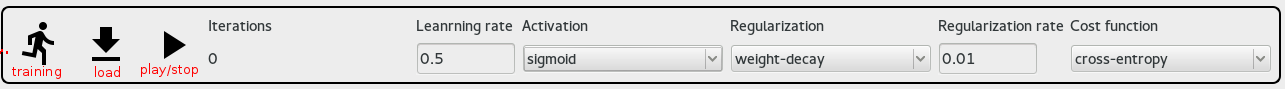
\includegraphics[scale=.4]{img/parametersLayer.png}
	\caption{Affichage des param\`etres d'activation}
\end{figure}

\paragraph{Choix des couches} La seconde couche permet de choisir les 3 types
de set de base de donn\'ees pour la couche d'entr\'ee (40,50,60 features), le
nombre de couches cach\'ees et le nombres de sortie du r\'eseau. Il est aussi
possible de choisir de d\'etecter le sexe de la personne ainsi que de choisir
un facteur multiplicatif pour la cr\'eation des neurones.

\paragraph{Choix du nombre de neurone} Cette troisi\`eme couche permet de
choisir un nombre de neurone illimit\'e pour chacune des couches du r\'eseau.

\paragraph{Affichage du r\'eseau} Cette derni\`ere couche permet de naviguer
entre 2 'Tab' afin de visualiser le r\'eseau ou les erreurs et les couts de
validation et d'entrainement (voir \ref{guinet} en annexe \ref{gui}).
\paragraph{L'affichage des couts et des erreurs} ce fait pendant que le
r\'eseau est entrain de de s'entrainer(voir \ref{guierr} en annexe \ref{gui}).

\subsection{Navigation}
Par d\'efault le r\'esau est configur\'e avec un taux d'apprentissage de 0.5,
une fonction d'activation SoftPlus, un taux de r\'egularisation de 0.01 et une
fonction de cout de type "cross-entropy". La couche d'entr\'ee poss\`ede par
default un un dataset de 40 multipli\'e par 15, une seule couche cach\'ee avec
50 neurones et 9 sorties. Ensuite les boutons d\'emarrer et pause permettent
de respectivement de d\'emarrer l'entrainement du r\'eseau ou de le stopper.



\section{Discussions}
\subsection{Problemes rencontr\'es}
Lors de l'entrainement du r\'eseau, nous avons d'abord \'et\'e confront\'e \`a
de tr\`es mauvaises performances. Nous avons initialement pens\'e que notre
pr\'e-traitement \'etait inefficace voir destructeur. En analysant les
performances plus en d\'etail,
nous nous sommes aper\c cu que le r\'eseau \'etait moins performant que si
nous lui faisions faire des pr\'edictions al\'eatoires
$\epsilon_{\bf x} \ge \left (1 - \frac{1}{9} = 88.9\% \right)$.
Ce qui est impossible et sugg\`ere que notre \'evaluation du co\^ut \'etait fausse.

En effet, nous avions commis une erreur dans la g\'en\'eration de nos vecteurs de
sortie. Lorsque la pr\'ediction \'etait compar\'ee \`a la sortie attendue,
celle-ci \'etait d\'ecal\'ee de 1 comme suit:
\begin{equation}
	\left (
	{\bf \hat y}_3 =
	\begin{bmatrix}
		0 \\
		0 \\
		{\color{red} 1 }\\
		0 \\
		0 \\
		0 \\
		0 \\
		0 \\
		0 \\
	\end{bmatrix}
	\right )
	\ne
	\left (
	{\bf y}_3 =
	\begin{bmatrix}
		0 \\
		0 \\
		0 \\
		{\color{red} 1 }\\
		0 \\
		0 \\
		0 \\
		0 \\
		0 \\
	\end{bmatrix}
	\right )
\end{equation}

\subsection{Conclusion et pistes d'am\'elioration}
Comme expliqu\'e pr\'ec\'edement, du \`a un manque de temps, nous avons
\'et\'e contrain de couper certaines optimisations notemment sur
l'impl\'ementation matricielle du {\em Mini-batch SGD}.

En revanche, malgr\'e cela, on observe tout de m\^eme de bonnes performances.
En utilisant comme r\'ef\'erence une classification de 9 digits en combinaison
avec une classification Homme/Femme (soit une sortie de 18 neurones) du
{\em TiDigits} dataset, on obtient un temps d'entrainement de 10 secondes sur un
{\em i5 dual-core, 2.2GHz} temps qui tombe \`a moins de 2 secondes sur un
{\em i7 quad-core, 4GHz}.

On remarque aussi une bonne capacit\'e de g\'en\'eralisation avec une erreur
d'environs 10-15\% sur le set de test apr\`es l'apprentissage.

En observant attentivement les matrices de
confusions en figure \ref{fig:w_prep} on remarque que le r\'eseau commet
principalement des erreurs lors de la classification Homme/Femme. Ceci pourrait
probablement \^etre du \`a un pr\'e-traitement trop {\em agressif} ou encore \`a
manque d'\'echantillons d'entrainement. Cette classification erron\'ee pourrai
peut-\^etre \^etre ajust\'ee en impl\'ementant une m\'ethode de
validation-crois\'ee plus avanc\'ee telle que le {\em V-folds} cit\'e pr\'ec\'edemment.

D'autres pistes d'am\'eliorations seraient d'ajouter la possibilit\'e de choisir une
fonctions d'activation diff\'erente pour la couche de sortie ou encore
l'impl\'ementation de techniques permettant de determiner {\em automatiquement}
les hyper-param\`eters du r\'eseau.


\newpage
\appendix
\section{Influences du pr\'e-traitement sur les performances du r\'eseau}
\begin{figure}[htp]
    \centering
    \subfloat{{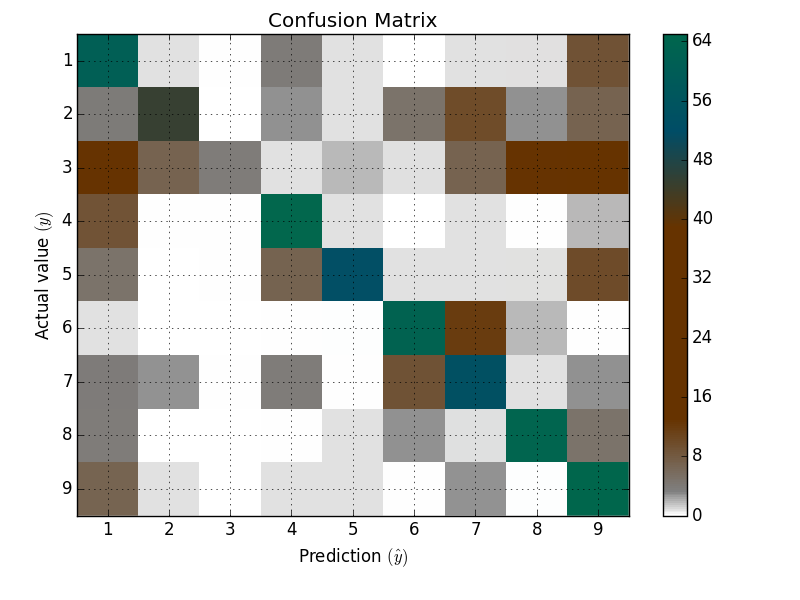
\includegraphics[width=.45\textwidth]{img/confusion_wo_prep.png} }}
    \subfloat{{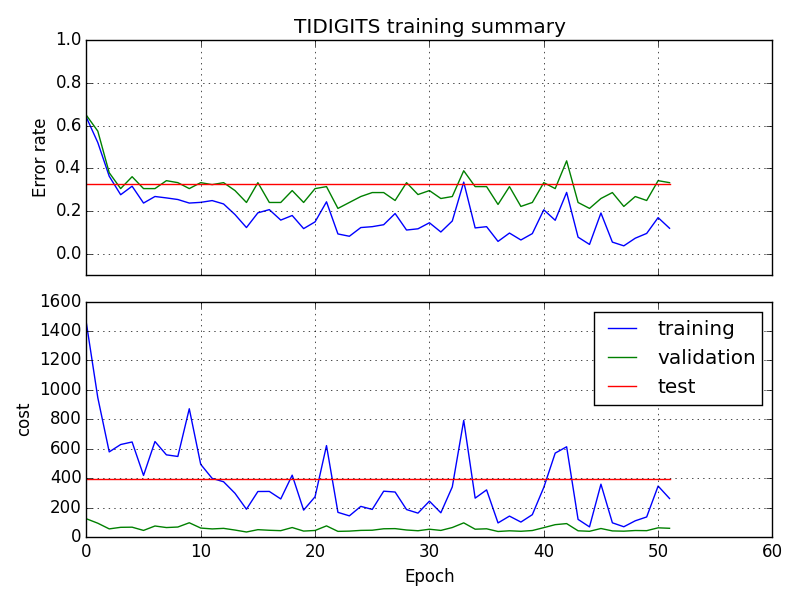
\includegraphics[width=.45\textwidth]{img/training_wo_prep.png} }}
    \caption{Performances sans pr\'e-traitement}
    \subfloat{{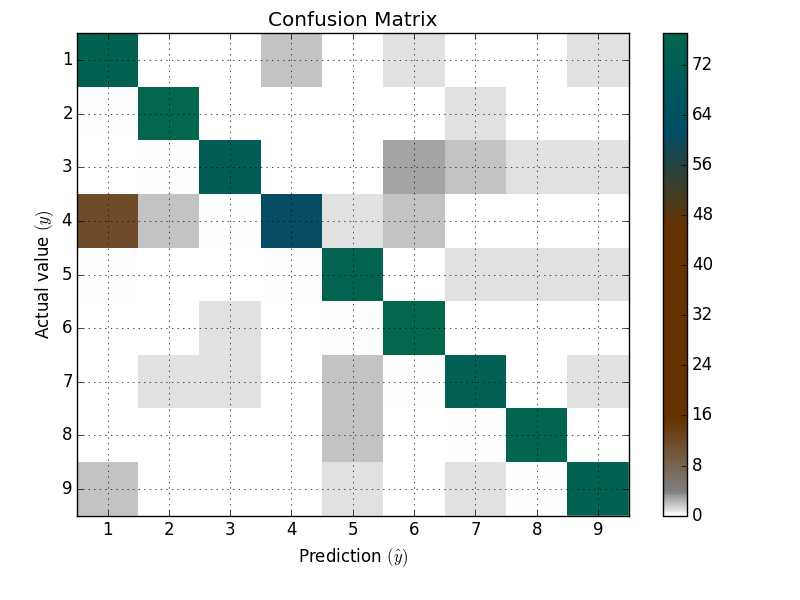
\includegraphics[width=.45\textwidth]{img/confusion_w_prep.png} }}
    \subfloat{{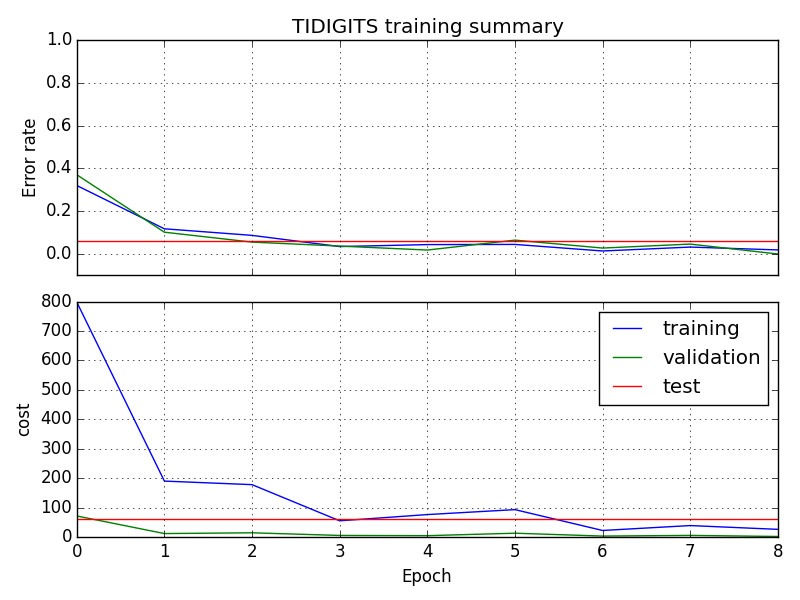
\includegraphics[width=.45\textwidth]{img/training_w_prep.png} }}
    \caption{Performances avec pr\'e-traitement}
    \label{fig:w_prep}
\end{figure}
\begin{figure}[htp]
    \centering
    \subfloat{{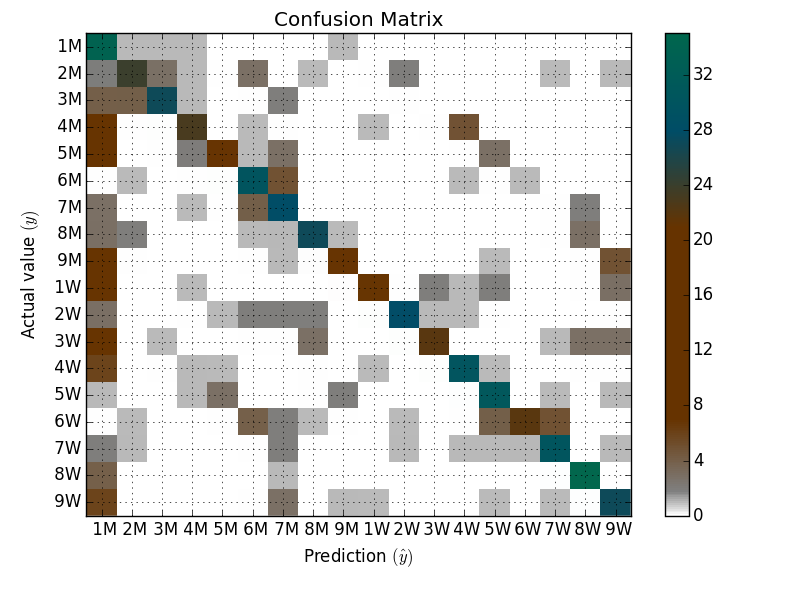
\includegraphics[width=.45\textwidth]{img/confusion_swo_prep.png} }}
    \subfloat{{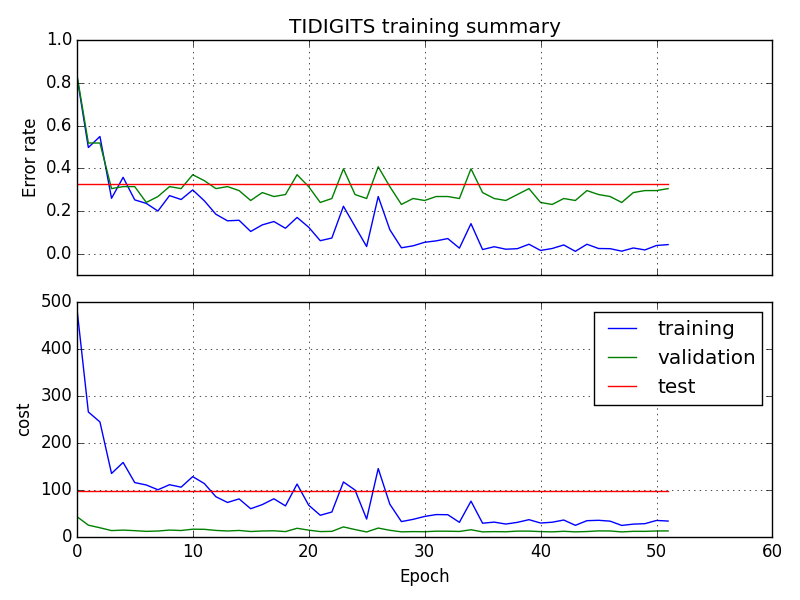
\includegraphics[width=.45\textwidth]{img/training_swo_prep.png} }}
    \caption{Performances sans pr\'e-traitement}
    \subfloat{{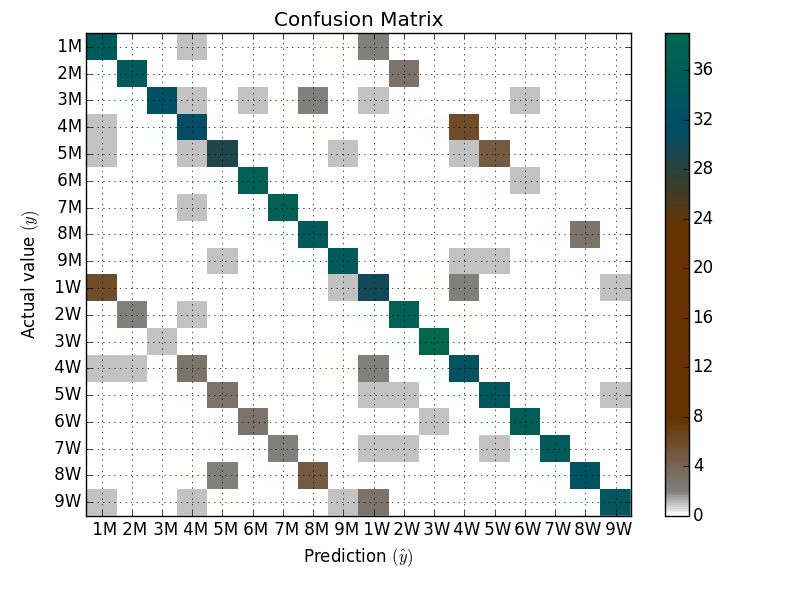
\includegraphics[width=.45\textwidth]{img/confusion_sw_prep.png} }}
    \subfloat{{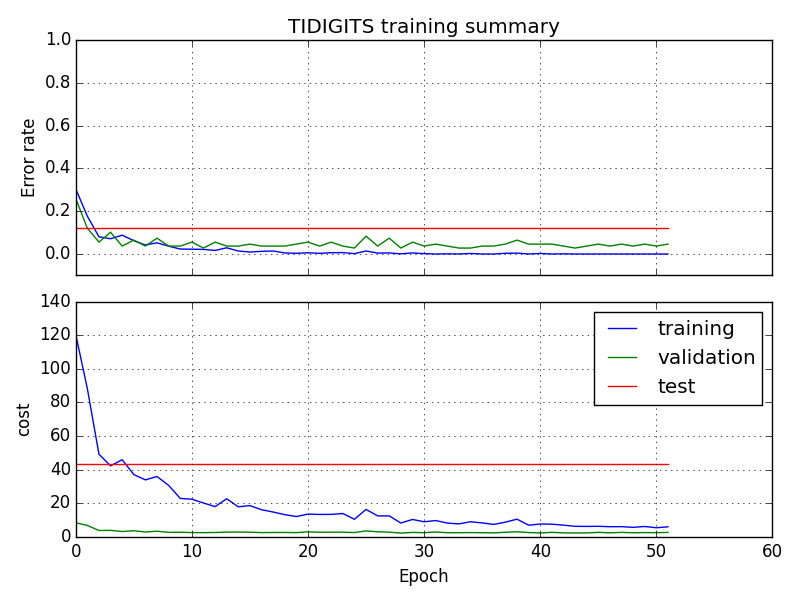
\includegraphics[width=.45\textwidth]{img/training_sw_prep.png} }}
    \caption{Performances avec pr\'e-traitement}
    \label{fig:w_prep}
\end{figure}
\newpage
\section{sauvegarde/chargement d'une configuration}
\label{saveload}
\lstset{tabsize = 4,
frame=lines,
numbers=none,
captionpos=b,
caption = {Sauvegarde et chargement interactif d'une configuration},
language = python,
basicstyle=\small}
\begin{lstlisting}
In [1]: import network as n
In [2]: my_net = n.Network([3, 4, 2], activation='sigmoid',
                   cost='cross-entropy', learning_rate=0.5)
In [3]: print my_net
Neural Network      : [3, 4, 2]
Activation function : sigmoid
Cost function       : cross-entropy
Regularization func : none
learning rate       : 0.5
Regularization rate : 0.1

L0  * * *
L1 * * * *
L2   * *
In [4]: my_net.save('foo.save')
In [5]: my_net = n.Network([8, 4, 4, 2], activation='tanh',
   ...:                   cost='quadratic', learning_rate=0.02,
   ...:				      regularization='L2', lambda_ = 0.001)
In [6]: print my_net
Neural Network      : [8, 4, 4, 2]
Activation function : tanh
Cost function       : quadratic
Regularization func : L2
learning rate       : 0.02
Regularization rate : 0.001

L0 * * * * * * * *
L1     * * * *
L2     * * * *
L3       * *
In [7]: my_net.load('foo.save')
In [8]: print my_net
Neural Network      : [3, 4, 2]
Activation function : sigmoid
Cost function       : cross-entropy
Regularization func : none
learning rate       : 0.5
Regularization rate : 0.1

L0  * * *
L1 * * * *
L2   * *
\end{lstlisting}

\newpage
\section{Inspection du r\'eseau}
\label{inspect}
\lstset{tabsize = 4,
frame=lines,
numbers=none,
captionpos=b,
caption = {Exemple d'inspection interactive d'un r\'eseau de neurones},
language = python,
basicstyle=\small}
\begin{lstlisting}
In [1]: import network as n
In [2]: my_net = n.Network((1, 2))
In [3]: my_net.load('foo.save')
In [4]: print my_net.struct
[3, 4, 2]

In [15]: print my_net.weights[0]
[[ 0.12737432  0.97734051 -0.56505148]
 [ 0.9090921   0.19178132 -0.15200818]
 [-0.07138651 -0.59903432 -0.78958921]
 [-0.55362229  0.51319807  0.2935551 ]]

In [16]: print my_net.weights[1]
[[-0.69519106  0.15539354 -0.46978019 -0.88703575]
 [-0.44994898 -0.57113777 -0.3736959  -0.00245537]]

In [17]: cat foo.save
# vim: set ft=yaml:
activation: sigmoid
biases:
- - [-0.920441751728251]
  - [-0.36244765002601287]
  - [-0.2926753984327689]
  - [-0.12034180777419923]
- - [1.1212748305651405]
  - [-0.565286303186786]
cost: cross-entropy
eta: 0.5
lambda: 0.1
regularization: none
struct: [3, 4, 2]
weights:
- - [0.12737431801447707, 0.9773405101355827, -0.5650514778232817]
  - [0.90909209744093, 0.19178132268834805, -0.1520081800115934]
  - [-0.07138650509286246, -0.5990343151487274, -0.7895892103519402]
  - [-0.5536222909987745, 0.5131980654305697, 0.29355509901743354]
- - [-0.6951910582048451, 0.1553935350379862, -0.4697801922017521,
		-0.8870357534796379]
  - [-0.44994897980803156, -0.5711377657299319, -0.3736959026341852,
		-0.002455368584577519]
\end{lstlisting}

\section{Visuels de l'interface graphique} \label{gui}
\begin{figure}[htp]
	\centering
	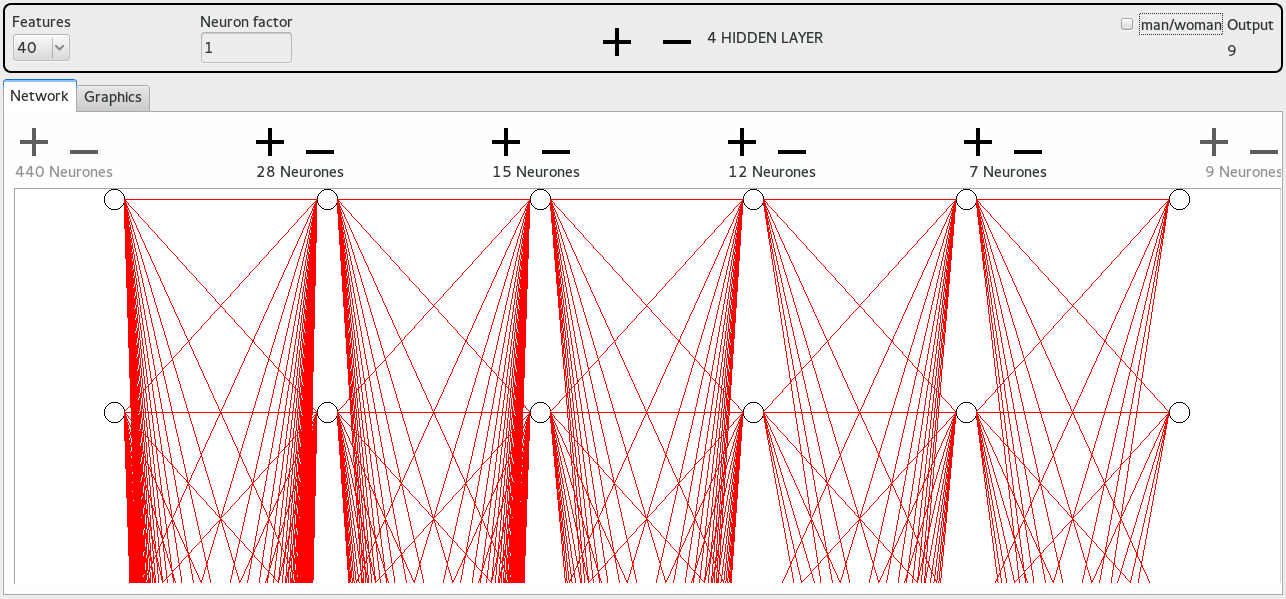
\includegraphics[scale=.27]{img/NetworkGraphics.png}
	\caption{Repr\'esentation visuelle du r\'eseau}
	\label{guinet}
\end{figure}

\begin{figure}[htp]
	\centering
	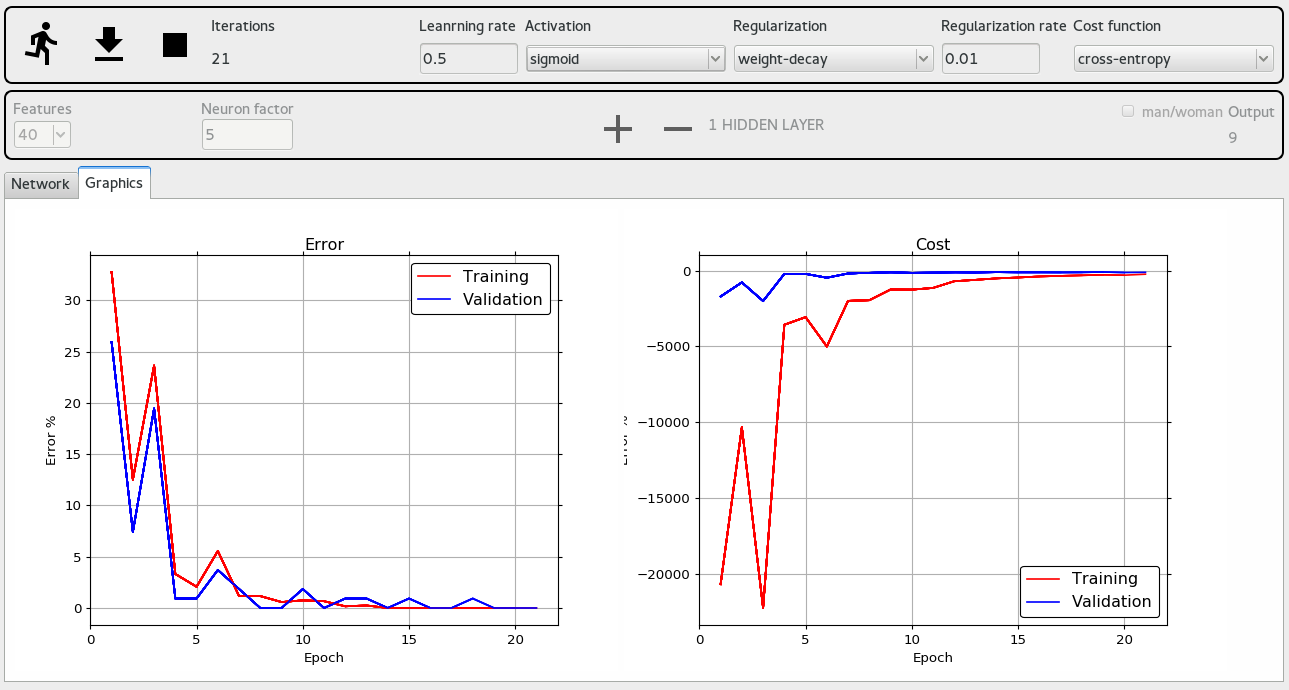
\includegraphics[scale=.27]{img/courbe.png}
	\caption{Affichage des courbes d'erreur et de co\^ut}
	\label{guierr}
\end{figure}


\end{document}
% vim: cc=80 :
